\documentclass[12pt] {article}
\usepackage[margin=1in]{geometry} %one inch margins
\usepackage{graphicx,color}
\renewcommand{\baselinestretch}{1.2} %double space, safe for fancy headers
\usepackage{pslatex} %Times font
\usepackage{apacite} %apa citation style
\bibliographystyle{apacite}
%\usepackage[pdfborder={0 0 0}]{hyperref}%for hyperlinks without ugly boxes
\usepackage{graphicx} %for figures
\usepackage{enumerate} %for lists
\usepackage{fancyhdr} %header
\usepackage{amssymb}
\pagestyle{fancy}
\usepackage[font={small,sf},format=plain,labelfont=bf,up]{caption}
\fancyhf{}
\fancyhead[l,lo]{Machine Learning \textit{ CS273A}} %left top header
\fancyhead[r,ro]{\thepage} %right top header
\begin{document}
\title{A comparison of three machine learning algorithms for predicting rainfall amount}
\author{Zachary DeStefano, Elmira Forouzmand, and Daniel Quang}
\date \today
\maketitle
\thispagestyle{empty}
\bigskip
%\tableofcontents
\pagebreak
\setcounter{page}{1}
\section{Introduction}
Regression is a common problem in the field of machine learning. It can be formulated as follows: Given some training data $D$, a set of $n$ points of the form $D=\{(\mathbf{x}_i,y_i) | \mathbf{x}_i \in \mathbb{R}^p, y_i \in \mathbb{R} \}$, find a prediction function $f$ that minimizes the error function. One additional constraint commonly encountered in regression problems is the requirement that all labels $y_i$ are non-negative. Typically, the error function is the mean-squared error (MSE): 
$$\frac{1}{n}\sum_{i=1}^n\left(f(\mathbf{x}_i)-y_i\right)^2$$
We explore three different machine learning algorithms: regression trees, Support Vector Regression (SVR), and neural networks, and compare their performance on predicting the amount of rainfall at a given location, using remote sensing (satellite) and numerical model data. 
\section{Materials and Methods}
\subsection{Data}
Training and testing data were downloaded from the in-class Kaggle competition, \textbf{How's the weather?}. The training dataset includes 60000 samples and the testing dataset includes 40000 samples. Labels are only available for training data, corresponding to non-negative rainfall amounts at various locations. Features are split into two sets: \textbf{X1} and \textbf{X2}. \textbf{X1} is a set of 91 primary features, and \textbf{X2} is a set of 441 features derived from raw IR3 local image patches.   

\subsection{Implementation}
The SVR algorithm was implemented in Python with the relevant modules from scikit-learn, an open source machine learning library. The regression trees algorithm was implemented in MATLAB using the class provided source codes.

The backpropagation algorithm for neural network training was implemented in Pylearn2, a machine learning Python library. Pylearn2 is built on top of Theano, another Python library that optimizes and stabilizes mathematical expressions and then compiles them to a GPU backend. The Pylearn2 Python codes were tested on Ubuntu Linux 14.04 with GCC 4.8.2, NVCC 6.5.12, and Python 2.7.9. Computations were performed using a machine with 6 Intel Xeon cores, an NVIDIA Titan Z graphics processor, and 64 GB memory.

\section{Results}
\subsection{SVR}
We first investigated the performance of the SVR algorithm. Briefly, the SVR algorithm is an optimization algorithm that works by minimizing the error while maximizing the margin. It has two hyperparameters to tune: $C$, the penalty for error, and $\gamma$, the threshold for tolerated error. Hyperparameter tuning was accomplished in a grid search fashion. Before training, \textbf{X1} and \textbf{X2} features are preprocessed by a Radial Basis Function Kernel. However, the SVR algorithm is generally very inefficient because its running time grows quadratically with the number of training samples. Therefore, we randomly selected 10000 training samples to train the model on, which we further split into a training and validation set in an 8:2 ratio. Based on the learning curves (\textbf{Figure 1}), we set $C$ and $\gamma$ to 1.2 and 5e-9, respectively. Evaluating this final model on the test dataset, we achieved an MSE of 0.444.

\renewcommand{\baselinestretch}{1.0} %double space, safe for fancy headers
\begin{figure}[h!] \centering
\begin{tabular}{cc}
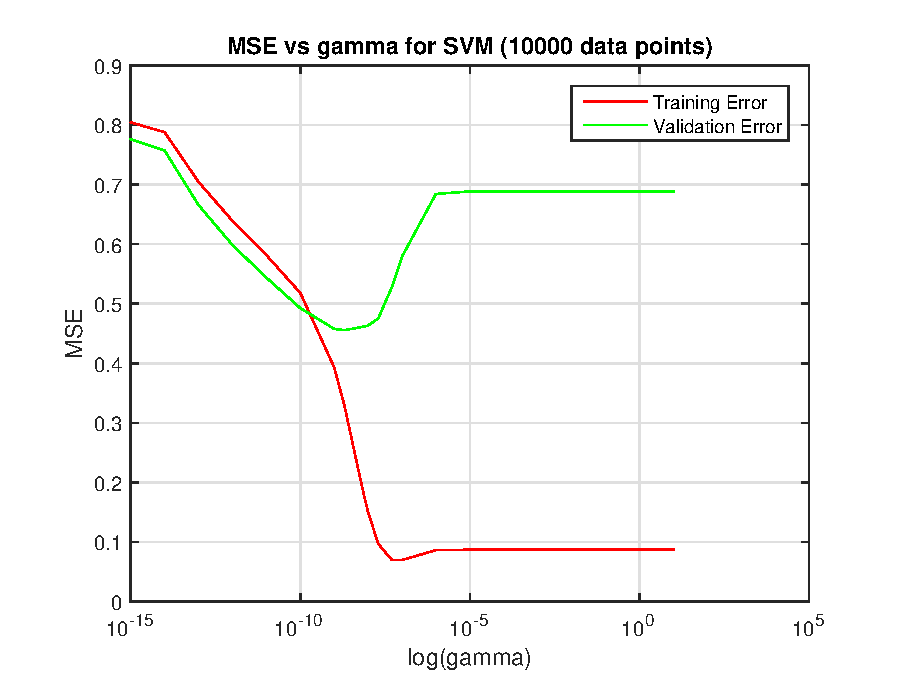
\includegraphics[width=.45\textwidth]{figdir/svmgamma10000.eps} &
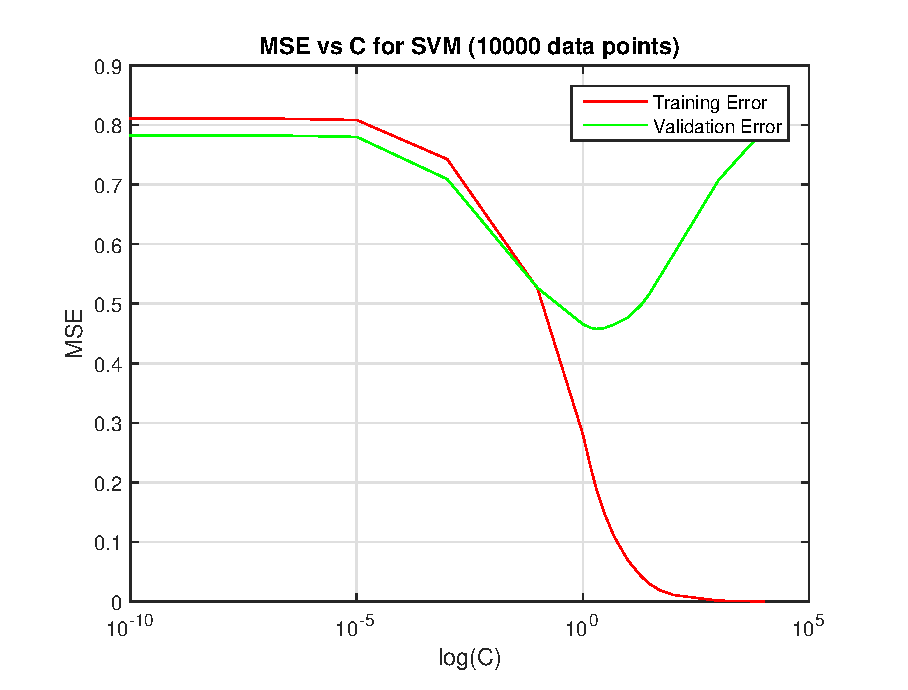
\includegraphics[width=.45\textwidth]{figdir/svmc10000.eps} \\
$C=1.5$ & $\gamma=5e-9$ \\
\end{tabular}
\caption{Learning curves for SVR showing the MSE (y-axis) on training data (red) and validation data (green) as a function of the hyperparameter $\gamma$ (left) or $C$ (right) (x-axis). Below each plot is the value of at which the other parameter is fixed.}
\end{figure}
\renewcommand{\baselinestretch}{1.2} %double space, safe for fancy headers


\subsection{Regression Trees}
Regression trees, or decision trees, can capture non-linear relationships among features and naturally output non-negative values. To develop our tree model, we first tune the hyperparameters, minParent and maxDepth, of a single decision tree (\textbf{Figure 2}) by evaluating its performance on 20\% of the training data we set aside as a validation set. The features include \textbf{X1} and the mean and standard deviation of the image patch features in \textbf{X2}. We find that setting the max depth and minParent to 20 and 512, respectively, provides optimal performance on the validation set.
\renewcommand{\baselinestretch}{1.0} %double space, safe for fancy headers
\begin{figure}[h!] \centering
\begin{tabular}{cc}
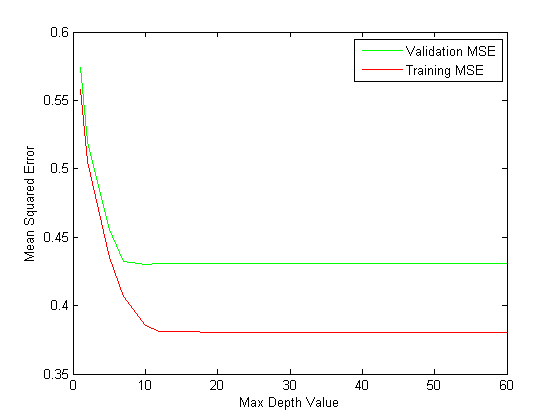
\includegraphics[width=.45\textwidth]{figdir/maxDepthVersusMSE.png} &
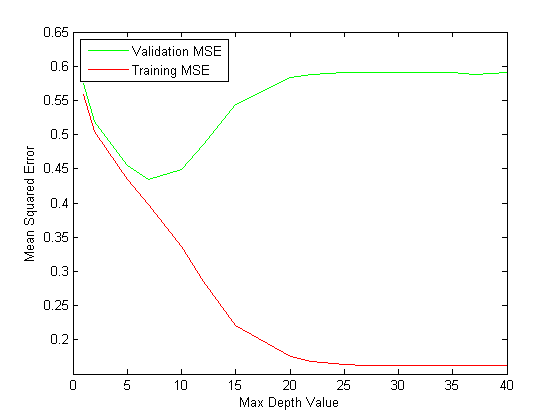
\includegraphics[width=.45\textwidth]{figdir/maxDepthVersusMSE2.png} \\
minParent=512 & minParent=32 \\
\end{tabular}
\caption{Learning curves for training a single decision tree showing the MSE (y-axis) on training data (red) and validation data (green) as a function of the max depth value (x-axis). Below each plot is the value minParent is fixed at.}
\end{figure}
\renewcommand{\baselinestretch}{1.2} %double space, safe for fancy headers
Although a single decision tree can perform well, an ensemble of decision trees can perform significantly better. We first investigate Random Forests, an ensemble method that averages outputs from decision trees trained on different feature subsets and random subsets of the training data (\textbf{Figure 3}). Our best Random Forest model (40 features and 60 weak learners) achieved an MSE of 0.363 on the test dataset. 

\renewcommand{\baselinestretch}{1.0} %double space, safe for fancy headers
\begin{figure}[h!] \centering
\begin{tabular}{cc}
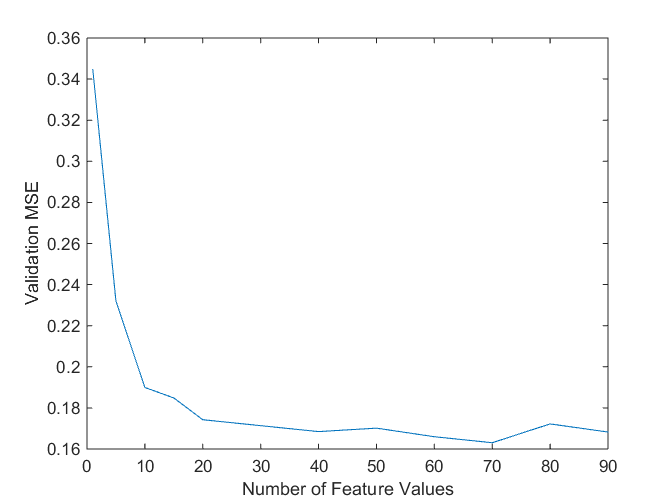
\includegraphics[width=.45\textwidth]{figdir/numFeatValuesVersusMSE.png} &
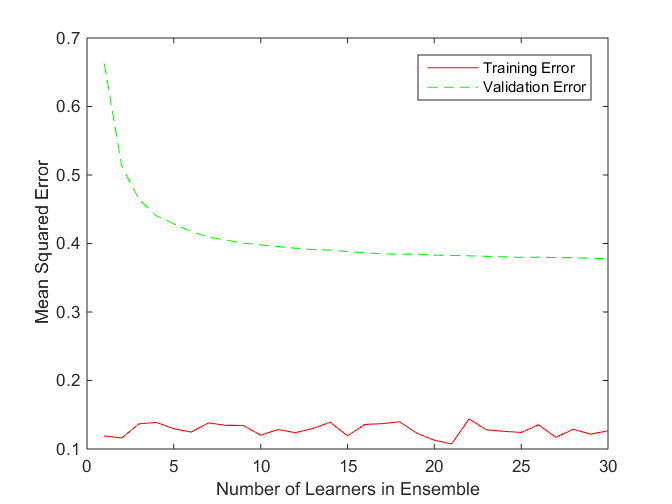
\includegraphics[width=.45\textwidth]{figdir/numLearnersVersusMSE.png} \\
\end{tabular}
\caption{Learning curves for training a random forest model. Plots show the MSE as either the number of feature values (left) or the number of learners in the ensemble (right) are varied. Max depth and MinParent of individual decision trees were set to 20 and 512, respectively.}
\end{figure}
\renewcommand{\baselinestretch}{1.2} %double space, safe for fancy headers

Next, we explored whether we can improve performance by combining Random Forests with Gradient Boosting, another ensemble method, according to the following procedure:
\begin{enumerate}
\item Train decision trees on random sets of 40 features
\item Take the 30 best sets of features and train boosted decision trees on them
\item Ensemble the trees from step 2
\end{enumerate}

\textbf{Figure 4} shows the learning curves for training the Gradient Boosted Random Forest. The ``best'' hyperparameters were selected and the model was retrained on the entire training dataset. This final model achieved an MSE of 0.378 on the test data, which is not an improvement on our Random Forest model.

\renewcommand{\baselinestretch}{1.0} %double space, safe for fancy headers
\begin{figure}[h!] \centering
\begin{tabular}{cc}
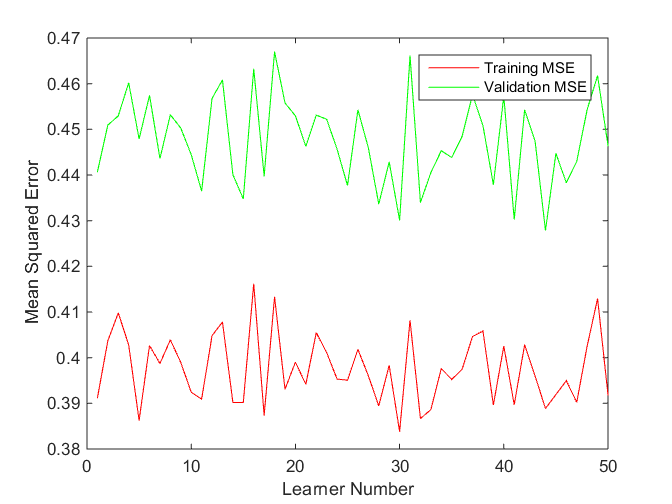
\includegraphics[width=.45\textwidth]{figdir/learnerNumVersusMSE.png} &
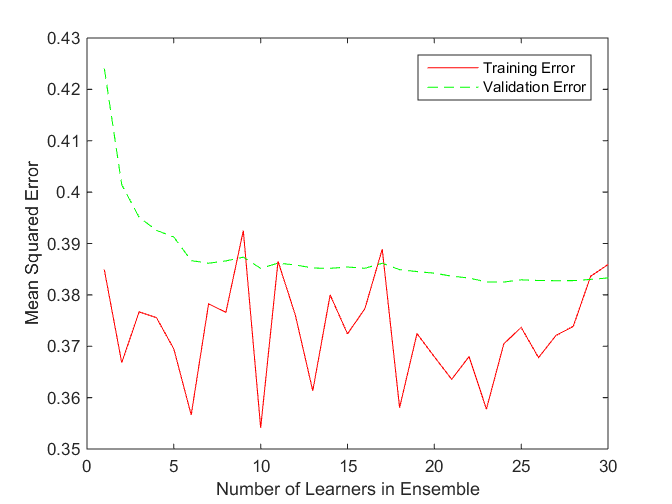
\includegraphics[width=.45\textwidth]{figdir/numLearnersVersusMSE2.png} \\
\end{tabular}
\caption{Learning curves for training a Gradient Boosted Random Forest. The left plot details gradient boosting and the right plot details the averaging of several models.}
\end{figure}
\renewcommand{\baselinestretch}{1.2} %double space, safe for fancy headers
\subsection{Neural Network}
We next trained a neural network to predict rainfall amounts. Briefly, neural networks are statistical learning algorithms inspired by biological neural networks in which interconnected ``neurons'' can compute values based only on the values of neighboring neurons. Deep learning is a branch of machine learning that explores the performance of stacking many hidden layers of neurons, through which multiple levels of abstraction can be inferred. This is advantageous for problems with many features because deep neural networks can infer the optimal set of features to use without any manual feature selection. Therefore, we trained neural networks on the full set of features, \textbf{X1} and \textbf{X2} (normalized to zero mean and unit variance). Neural networks have recently become more popular due to their state-of-the-art performances in machine learning problems such as image and speech recognition, the development of advanced deep learning techniques such as dropout and unsupervised pretraining, and the application of powerful parallelized graphical processing units.

To study how deeper networks perform, we trained neural networks with between 1 and 5 hidden layers (data for model with 4 hidden layers not shown). Due to the large number of parameters, neural networks have a tendency to overfit if trained for too many training steps or epochs. Therefore, we further split the training data into a training and validation set in a 9:1 ratio. Training is terminated if the validation MSE, which is evaluated at the end of each training epoch, fails to decrease after 10 training epochs. Each hidden layer contains 1000 hidden neurons and the learning rate is fixed at 0.001. Rectified linear units serve as the activation function for computing the values of the hidden neurons and the final output layer is a standard linear layer. All weights were initialized by randomly drawing from a Gaussian distribution with mean 0 and standard deviation 0.01. Weights were updated by stochastic gradient descent with a fixed minibatch size of 100.

Learning curves for the neural network training clearly displays evidence of overfitting (\textbf{Figure 5}). Optimal performance on the validation was reached around 122 training epochs. Based on the performance on the validation set, we selected the neural network with 2 hidden layers as our ``best'' model. We retrained this neural network with the full training data for 122 epochs and evaluated. Because linear output layers are not strictly non-negative, we apply an additional preprocessing step of converting all negative predictions to 0 before evaluating the trained model on the testing set. Evaluating this model on the test data, we achieved an MSE of 0.364.
\renewcommand{\baselinestretch}{1.0} %double space, safe for fancy headers
\begin{figure}[h!] \centering
\begin{tabular}{cc}
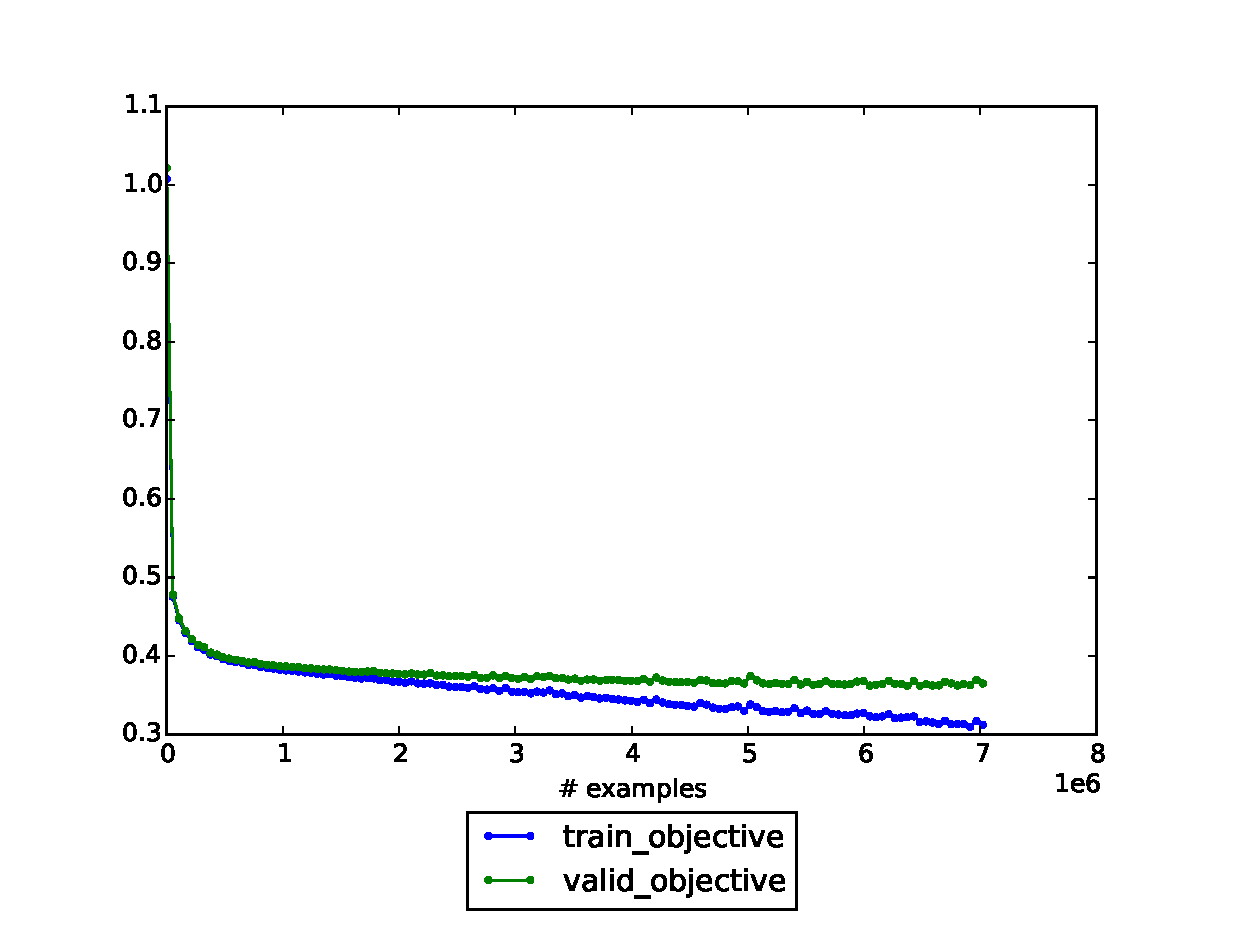
\includegraphics[trim = 0mm 20mm 0mm 10mm, clip=true, width=.45\textwidth]{figdir/nn_mse_1.eps} &
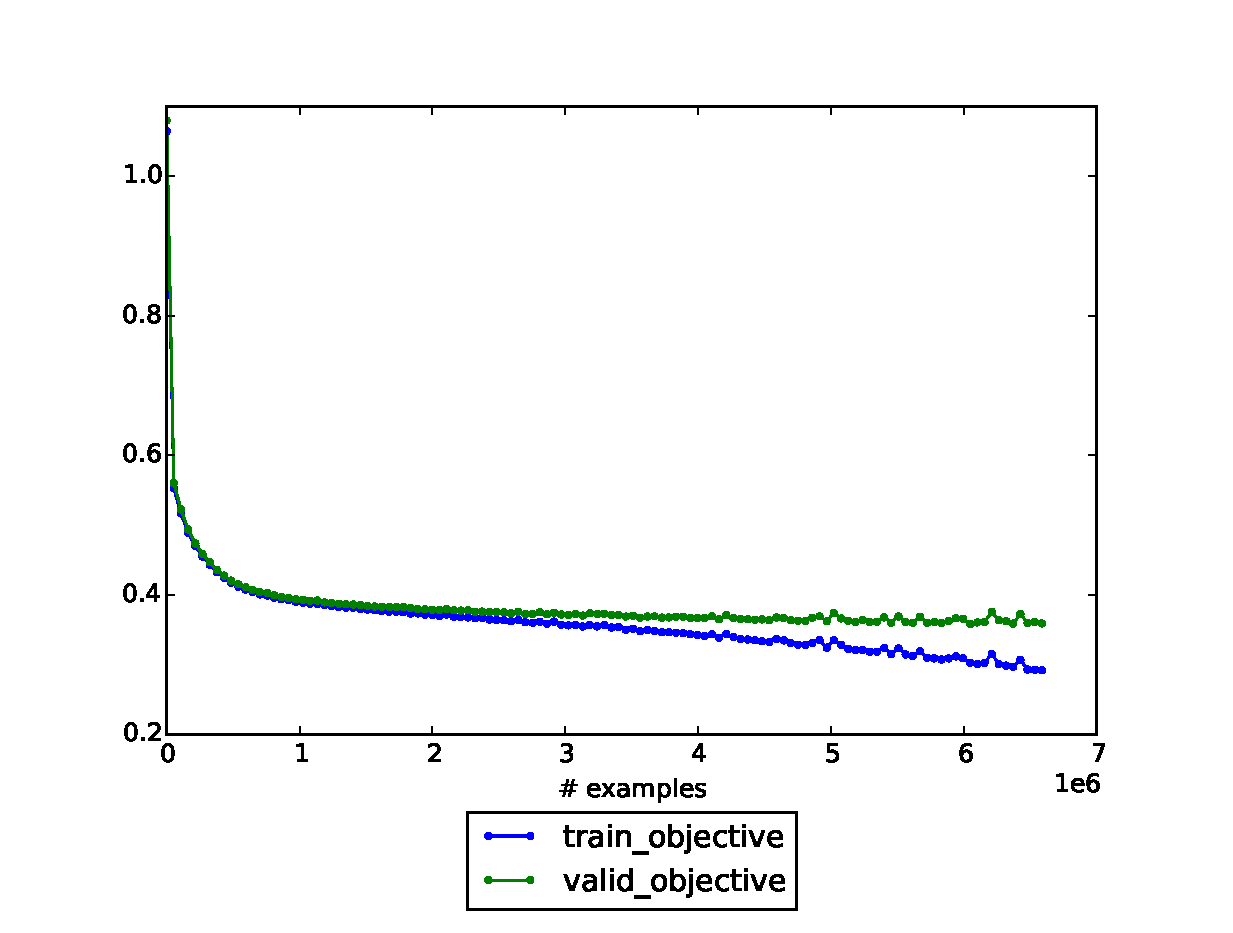
\includegraphics[trim = 0mm 20mm 0mm 10mm, clip=true, width=.45\textwidth]{figdir/nn_mse_2.eps} \\
$N_{hidden}=1$ & $N_{hidden}=2$ \\
Train MSE: $0.316$ & Train MSE: $0.303$ \\
Validation MSE: $0.362$ & Validation MSE: $0.358$ \\
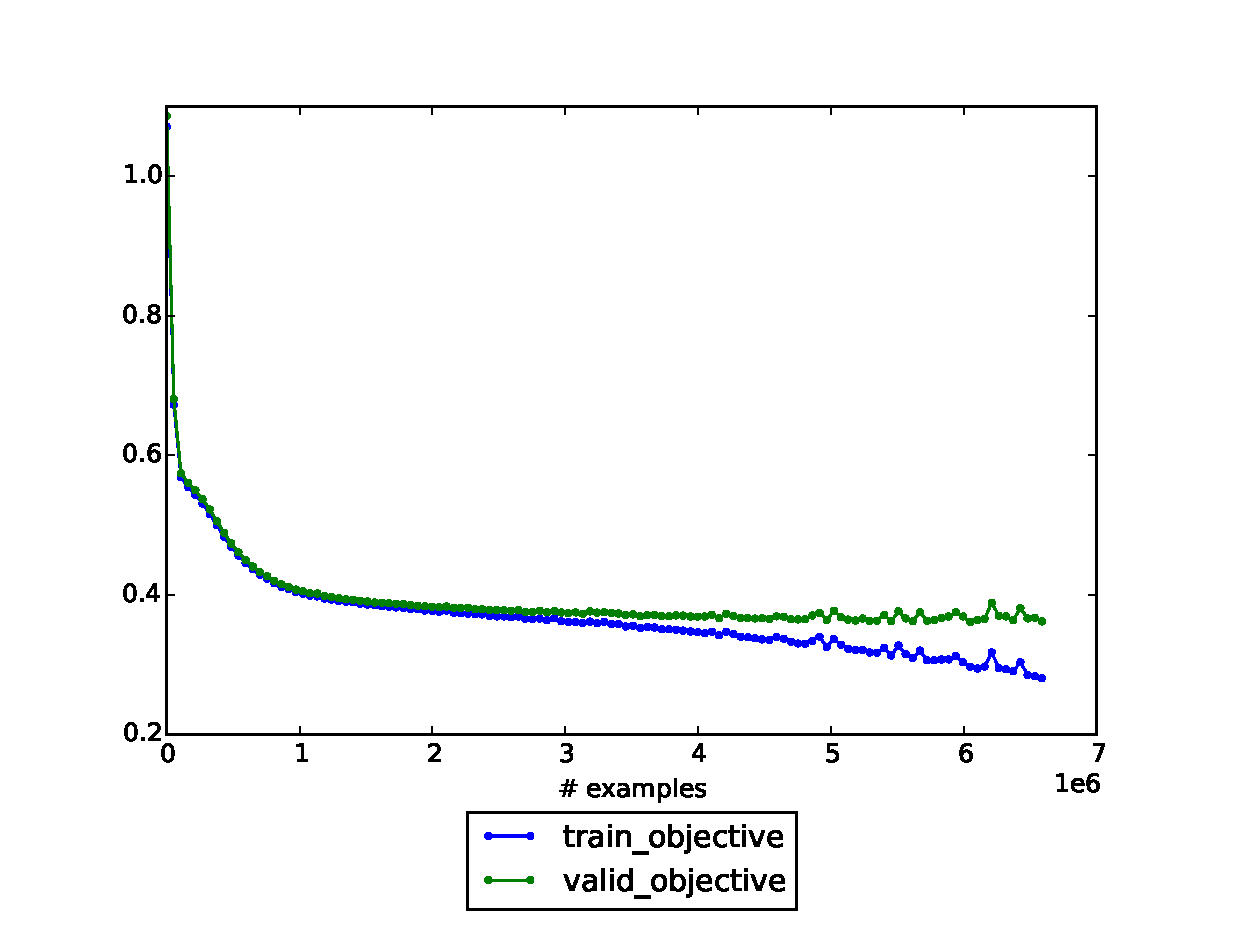
\includegraphics[trim = 0mm 20mm 0mm 10mm, clip=true, width=.45\textwidth]{figdir/nn_mse_3.eps} &
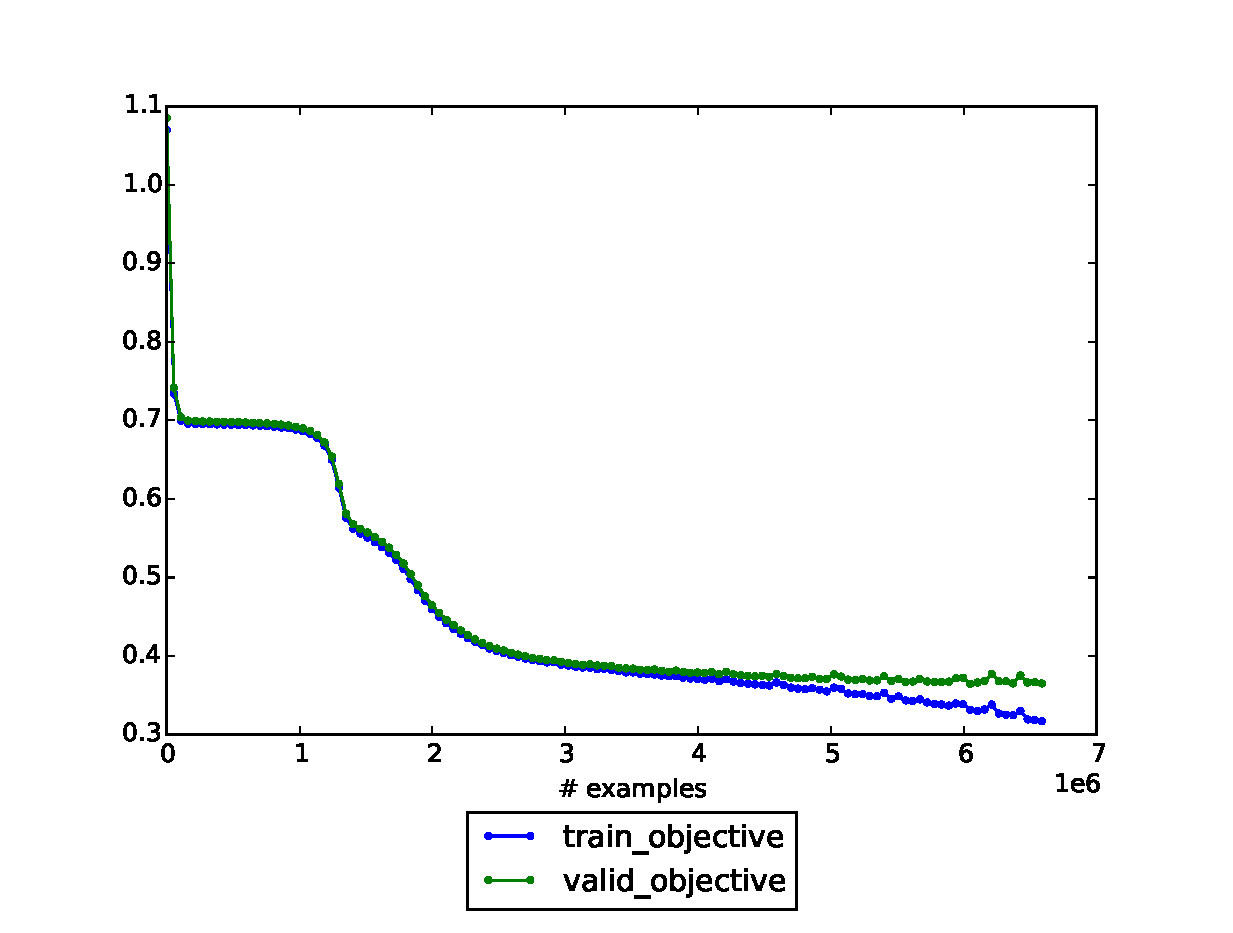
\includegraphics[trim = 0mm 20mm 0mm 10mm, clip=true, width=.45\textwidth]{figdir/nn_mse_5.eps} \\
$N_{hidden}=3$ & $N_{hidden}=5$ \\
Train MSE: $0.297$ & Train MSE: $0.332$ \\
Validation MSE: $0.361$ & Validation MSE: $0.365$ \\
\end{tabular}
\caption{Learning curves for neural network training showing the MSE (y-axis) on training data (blue) and validation data (green) as a function of the number of training samples processed (x-axis). Below each plot is the number of hidden layers in the neural network, and the training and validation MSE of the model yielding the lowest validation MSE during training.}
\end{figure}
\renewcommand{\baselinestretch}{1.2} %double space, safe for fancy headers

\subsection{Summary of results on test data}
\textbf{Table 1} summarizes the performance of the three models on the test dataset. We find that regression trees perform the best overall, but neural networks perform similarly well, while SVR performs the worst.
\begin{table}\centering
\begin{tabular}{cccc}
& SVR & Random Forest & Neural Network \\
\hline
Test MSE & 0.444 & 0.363 & 0.364
\end{tabular}
\caption{Summary of performance on testing data with three models.}
\end{table}
\section{Discussion and conclusions}
In this paper, we tuned and compared three different machine learning regression models and compared their performance on predicting rainfall amounts. Based on the MSE on the test data, SVR performs the worst, while regression trees and neural networks achieve very similar performance. Future work can focus on improving the individual models. For SVR, one of the limiting factors was that we had to train on a subset of the data due to the long running time of the training algorithm. An obvious route to explore is to apply powerful GPU hardware to accelerate SVR training so that we can train an SVR model on the entire training dataset. Based on the overfitting observed in the neural network training, we can explore how dropout improves performance. Applying momentum training, which adjusts the learning rate throughout training, is another option. Different ensemble strategies for regression trees, such as AdaBoost and Extra Trees, may also improve performance. Another avenue of future interest is to combine results from multiple models, including the 3 models considered in this paper, into an ensemble model.

\section{Authors' contributions}
All authors wrote the manuscript. ZD implemented regression trees. EF implemented SVR. DQ implemented neural networks. All authors read and approved the final manuscript.
\end{document}